\documentclass[12pt, twoside, letterpaper]{report}
\usepackage[top=2cm,bottom=4cm,left=3cm,right=3cm,asymmetric]{geometry}

\usepackage{fancyhdr}
\pagestyle{fancy}
\fancyfoot[C]{}    
\fancyfoot[LE,RO]{\thepage}        
\fancyhead[RO]{\slshape \rightmark}        
\fancyhead[LE]{\slshape\leftmark}      
\fancyhead[RE,LO]{}  

\usepackage{color}   
\usepackage{hyperref}
\usepackage[utf8x]{inputenc}
\usepackage[italian]{babel}
\usepackage{amsmath, amsthm, amssymb, amsfonts}
\usepackage[breakable]{tcolorbox}
\usepackage{pdfpages}
\usepackage{enumitem}
\usepackage{caption}
\usepackage{subcaption}
\usepackage{graphicx}
\graphicspath{ {./img/} }
\newcommand{\img}[4] {
	\begin{figure}[h]
		\caption{#1}
		\centering
		\includegraphics[scale=#2]{#3}\\
		\label{#4}
	\end{figure}
}

\title{Uso di reti neurali per la classificazione di dati in problemi di medicina legale}
\author{Mario Petruccelli \cr Università degli studi di Milano}
\date{A.A. 2019/2020}

\begin{document}

	\begin{titlepage}
		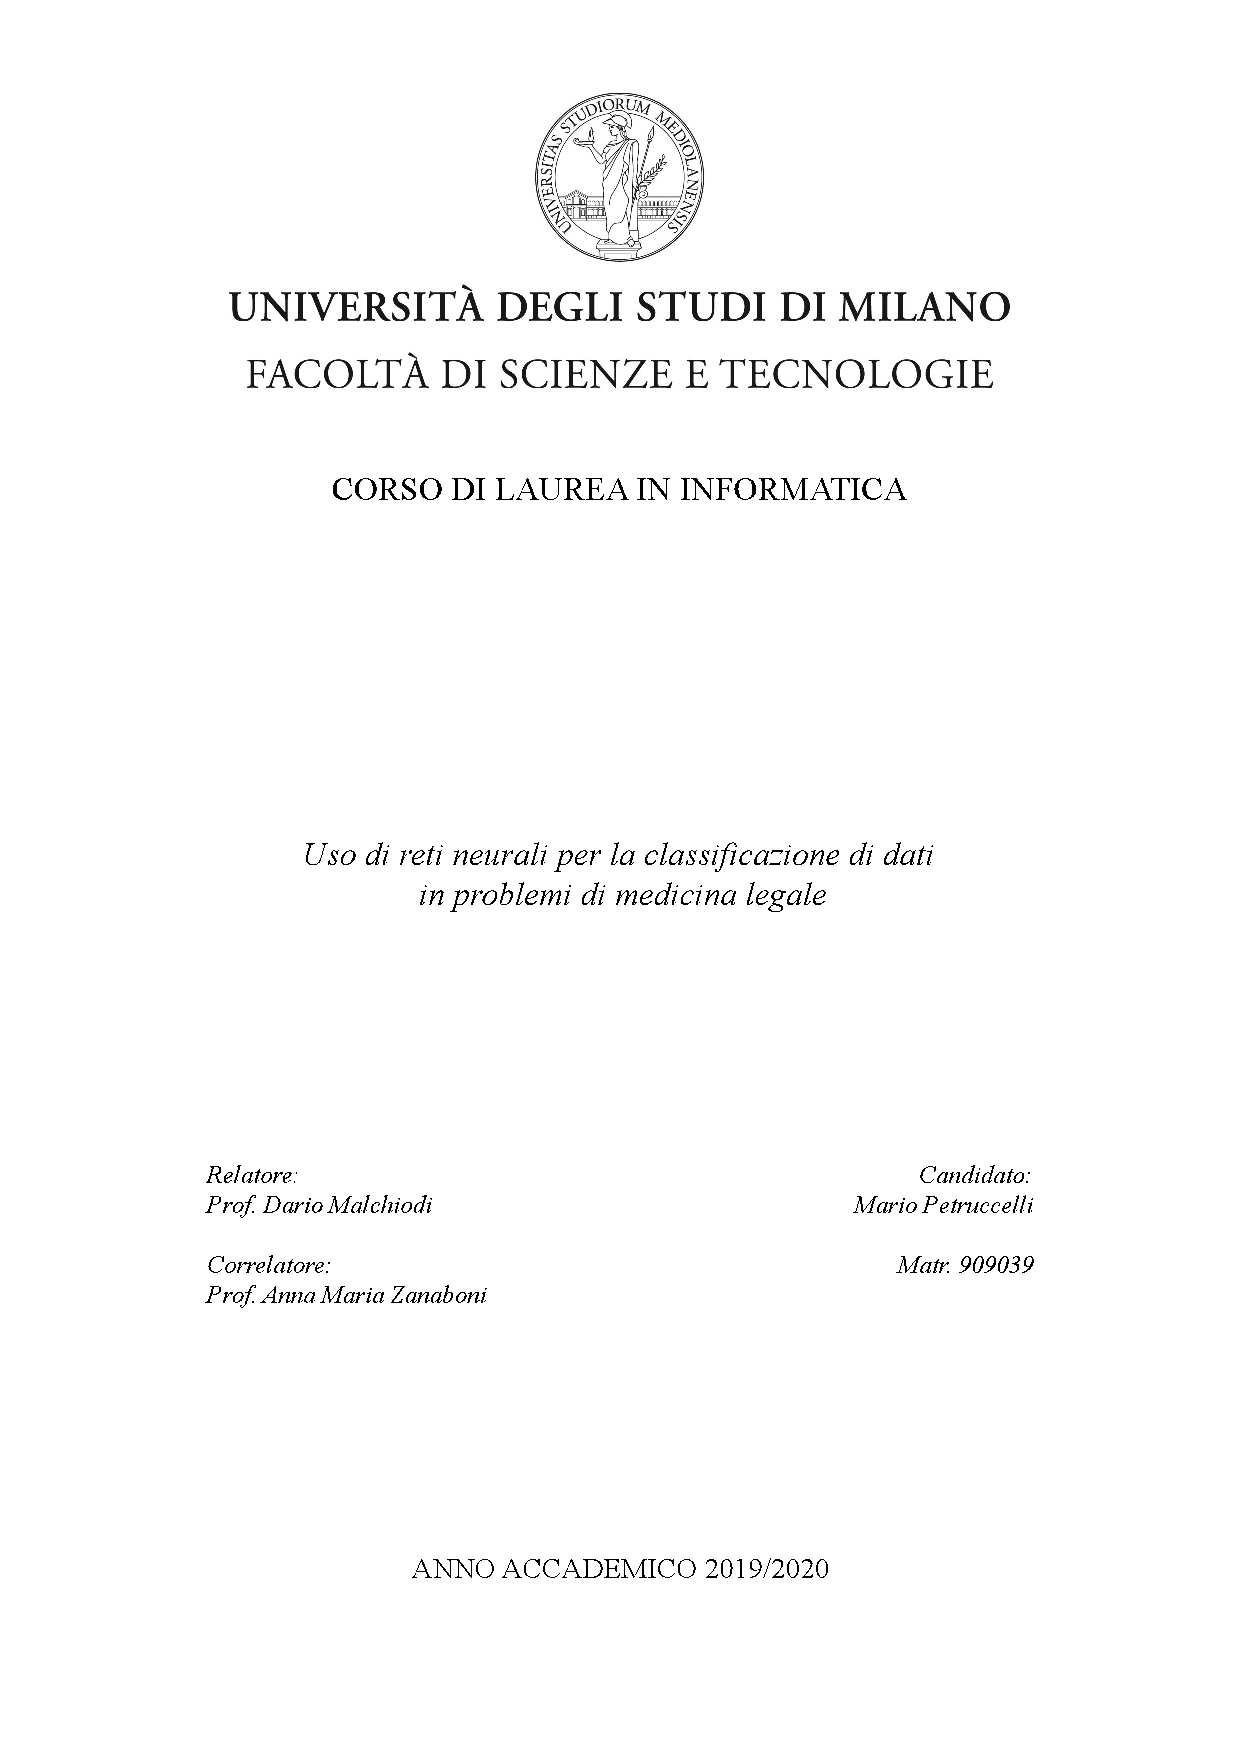
\includepdf{img/FRONTESPIZIO.pdf}
		\newpage
		\tableofcontents
	\end{titlepage}

	\chapter*{Introduzione} \markboth{Introduzione}{}
		Qua ci andrà l'introduzione

		\newpage		
	\chapter{Reti neurali}
		Le \textbf{reti neurali artificiali} sono un campo molto importante del \textit{machine learning}. Consistono in un modello matematico che prende ispirazione dalle reti neurali biologiche, presenti nel cervello animale. In questo capitolo ne vedremo le loro componenti e il loro funzionamento. Ma cos'è il machine learning?

		\section{Paradigma del machine learning}
			Il machine learning è una disciplina scientifica dell'ambito dell'intelligenza artificiale ed è una di quelle in più rapida espansione; negli ultimi decenni è diventato di uso comune in moltissime applicazioni che richiedono l'estrazione di informazioni da dati su larga scala. Lo scopo di tale disciplina è quello di individuare dei pattern significativi nei dati, che difficilmente sarebbero riconoscibili con l'uso tradizionale della programmazione \textit{(e.g. riconoscere la razza di un cane partendo da una foto)}.  
			
			Prendendo come esempio noi umani, molte delle nostre abilità vengono acquisite o raffinate dalla nostra esperienza, e così \textit{impariamo}. Immaginiamo di trovarci in un'isola sperduta e di trovare un albero con frutti mai visti prima. Nonostante questo frutto sia nuovo ai nostri occhi, sapremo riconoscere con molta probabilità se è maturo o acerbo. Lo stesso concetto possiamo provare ad applicarlo alle macchine, ma come possono apprendere? 
			
			\subsection{Tipi di apprendimento} L'apprendimento è un dominio di ampio spettro e di conseguenza, il machine learning è diviso in diversi sottocampi in cui abbiamo più paradigmi di apprendimento. La principale distinzione che possiamo fare è la differenza tra l'apprendimento \textbf{supervisionato} e \textbf{non supervisionato}.
			
				\paragraph{Apprendimento supervisionato} Consideriamo di dover classificare tre specie di fiori leggermente diversi tra loro, appartenenti alla stessa famiglia \textit{(esperimento che riprenderemo più avanti)}. Per imparare a riconoscerli, potremmo ricevere un insieme di dati \textit{(e.g. larghezza dei petali, lunghezza del gambo, ecc...)} appartenenti ai fiori di cui conosciamo già l'etichetta. Dopo questa fase di \textbf{allenamento}, dovremmo essere in grado di trovare un pattern tra i dati per etichettare nuovi fiori, questa volta privi di etichetta e non appartenenti all'insieme dato in precedenza. 
				
					In maniera più astratta, possiamo vedere questo come un processo di \textit{utilizzo dell'esperienza passata per acquisire competenza}. L'apprendimento supervisionato descrive uno scenario in cui l'esperienza, nel nostro caso un insieme di \textbf{training}, contiene delle etichette che non sono presenti nell'insieme di \textbf{test}, a cui dobbiamo applicare l'esperienza acquisita in modo da \textbf{predire} l'informazione mancante.
				
				\paragraph{Apprendimento non supervisionato}  Nell'apprendimento non supervisionato non c'è distinzione tra i dati di training e di test. Vengono processati i dati con lo scopo di tirare fuori una versione compressa, o un "riassunto" di essi. Il raggruppamento dei dati in sottoinsiemi con caratteristiche simili è una delle pratiche più usate in questo campo.\\
				
				Il modello di cui ci occuperemo noi, ovvero le reti neurali artificiali, utilizzano un'apprendimento di tipo supervisionato. Andiamo a vederle più nel dettaglio.
			
		\section{Che cos'è una rete neurale?}
			Come abbiamo già anticipato, le reti neurali artificiali cercano di riprendere quello che sono le loro omonime biologiche. Il cervello animale è un meccanismo in grado di apprendere grazie all'esperienza, ed è per questo che si è cercato di emularlo \textit{(in modo molto semplificato)} come modello di machine learning. Probabilmente saprete già che il cervello è composto da \textbf{neuroni}, ed essi sono connessi tra di loro da delle \textbf{sinapsi} in modo da poter comunicare. Ebbene, anche il nostro modello artificiale riprende questa struttura.
			
		\subsection{Componenti principali di una rete neurale} 
			\paragraph{Concetto di tempo} Prima di dare una definizione, introduciamo il concetto di tempo in una rete neurale. Ci si riferisce al tempo vigente come $(t)$, al passo successivo come $(t+1)$, al passo precedente come $(t-1)$, e così via.
			\paragraph{Rete neurale artificiale}
			Una rete neurale artificiale può essere vista come un grafo, cioè consiste in un insieme di \textbf{nodi} \textit{(neuroni)} e \textbf{archi orientati pesati} \textit{(sinapsi)}. Più formalmente, una rete neurale è una tripla $(N,V, \omega)$ in cui:
			\begin{itemize}
				\item $N$ è l'insieme dei neuroni.
				\item $V = \{(i,j) | i,j \in N\}$ è l'insieme delle connessioni tra i neuroni $i$ e $j$.
				\item $\omega: V \rightarrow \mathbb{R}$ è la funzione di peso, dove $\omega_{i,j}$ è il peso della connessione tra i neuroni $i$ e $j$.
			\end{itemize}
			Un neurone, per essere definito tale deve essere in grado di elaborare i dati che gli arrivano tramite le sue connessioni. È composto da tre funzioni: funzione di \textbf{propagazione}, funzione di \textbf{attivazione} e funzione di \textbf{uscita}. 
			
			\img{Struttura di un neurone}{0.4}{neurone.png}{neurone}
			
			 \paragraph{Funzione di propagazione} Dato un neurone $j$, la sua funzione di propagazione riceve gli output $o_{i_1}, \dots, o_{i_n}$ dei neuroni $i_1, \dots, i_n$ connessi a $j$ e i corrispettivi pesi $\omega_{i,j}$, restituendo un valore detto \textit{network input} net$_j$ che verrà poi processato dalla \textit{funzione di attivazione}. 
			 
			 	Sia $I = \{i_1, i_2, \dots, i_n\}$ l'insieme dei neuroni tale che $\forall z \in \{1, \dots, n\} : \exists w_{i_z,j}$. Allora il network input di $j$ ($net_j$), è calcolato dalla funzione di propagazione $f_{prop}$ come segue: $$net_j = f_{prop}(o_{i_1}, \dots, o_{i_n},w_{i_1,j}, \dots, w_{i_n,j})$$
			 	La funzione di propagazione più usata è la \textbf{somma pesata}, ovvero la somma delle moltiplicazioni dell'output di ogni neurone $i$ per il corrispettivo peso $\omega_{i,j}$: $$net_j = \sum_{i \in I} o_i w_{i,j}$$
			 	
			 \paragraph{Stato di attivazione e valore di soglia} Così come in natura, un neurone può essere \textit{attivo} o meno. Lo \textbf{stato di attivazione} \textit{(o attivazione)} è una reazione ai valori che abbiamo ricevuto in input, e il neurone viene attivato quando il \textit{network input} supera il \textbf{valore di soglia} di quel neurone. Sia $j$ un neurone. Il \textbf{valore di soglia} $\Theta_j$ è assegnato unicamente a $j$ e indica la posizione del valore massimo del gradiente della funzione di attivazione.
			 
			 \paragraph{Funzione di attivazione} Sia $j$ un neurone. La funzione di attivazione è così definita: $$a_j(t) = f_{act}(net_j(t),a_j(t-1), \Theta_j)$$
			 	Trasforma il \textit{network input} net$_j$, il precedente stato di attivazione $a_j(t-1)$, e il valore di soglia $\Theta_j$ in un nuovo stato di attivazione $a_j(t)$ 
			 	A differenza di molte delle variabili definite prima, la funzione di attivazione viene definita \textit{globalmente} per tutti i neuroni. Esistono diverse funzioni di attivazione, alcune tra le più usate, come possiamo vedere in figura~\ref{fig:funzioni di attivazione} sono: 
			 	\begin{itemize}
			 		\item La funzione logistica: $f(x) = \frac{1}{1+e^{-x}}$
			 		\item La funzione tangente iperbolica: $f(x) = tanh(x)$
			 		\item La funzione ReLU: $f(x) = max(0,x)$
			 		\item La funzione identità: $f(x) = x$
			 	\end{itemize}
			 	
			 \begin{figure}
				\begin{subfigure}[]{.5\textwidth}
					\centering
					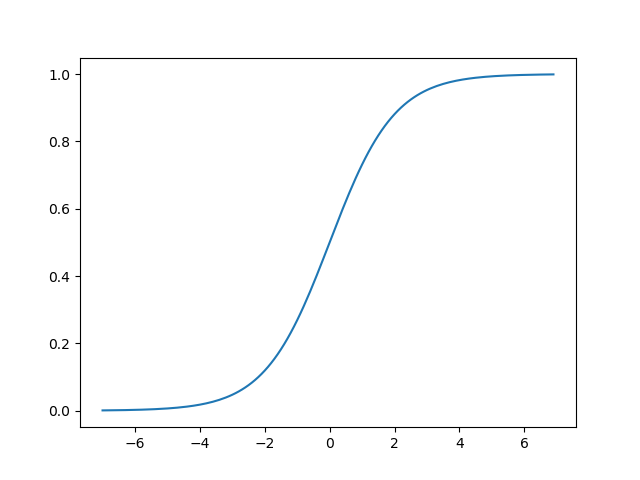
\includegraphics[width=0.7\linewidth]{logistic.png}
					\caption{Funzione logistica}
					\label{fig:logistic}
				\end{subfigure}
				\hfill
				\begin{subfigure}[]{.5\textwidth}
					\centering
					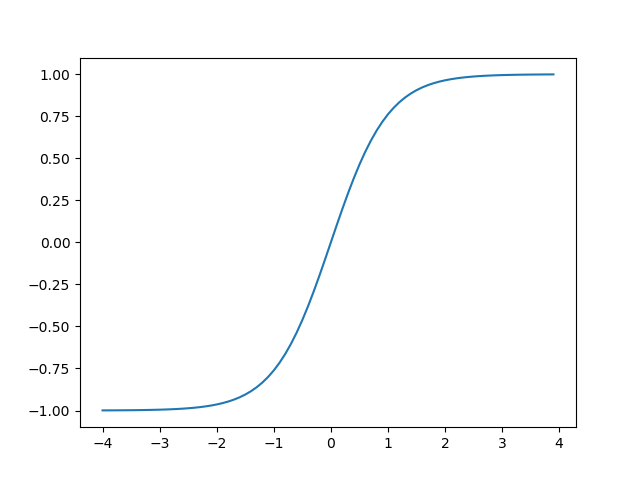
\includegraphics[width=0.7\linewidth]{tanh.png}
					\caption{Funzione tangente iperbolica}
					\label{fig:tanh}
				\end{subfigure}
				
				\bigskip  
				
				\begin{subfigure}[]{.5\textwidth}
					\centering
					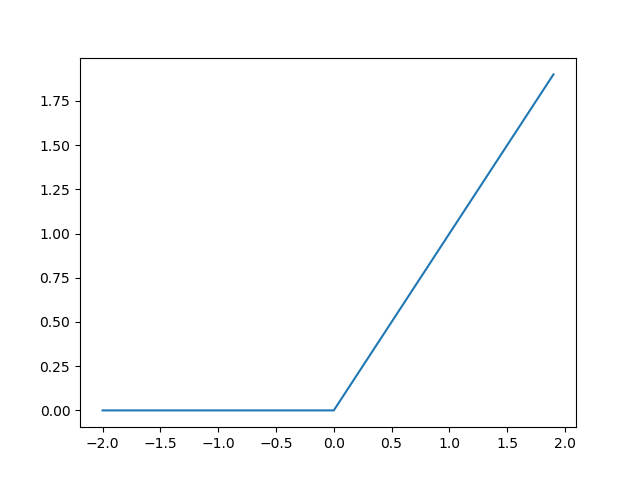
\includegraphics[width=0.7\linewidth]{relu.png}
					\caption{Funzione ReLU}
					\label{fig:relu}
				\end{subfigure}
				\hfill
				\begin{subfigure}[]{.5\textwidth}
					\centering
					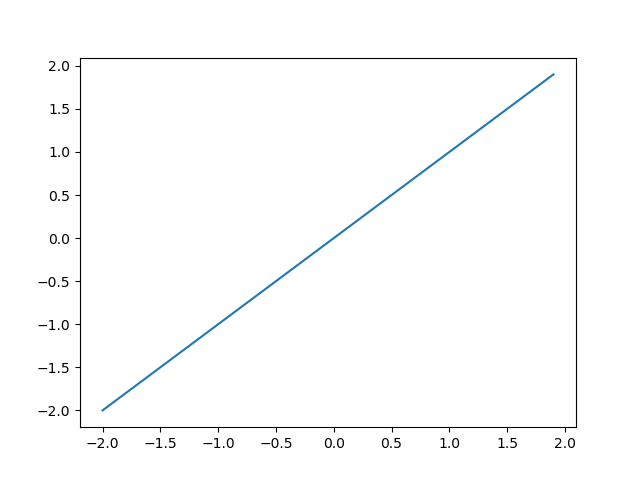
\includegraphics[width=0.7\linewidth]{identity.png}
					\caption{Funzione di identità}
					\label{fig:identity}
				\end{subfigure}
				
				\caption{Funzioni di attivazione}
				\label{fig:funzioni di attivazione}
			\end{figure}	
			 	
			 \paragraph{Funzione di uscita} La funzione di uscita di un neurone $j$ calcola i valori che verranno trasmessi agli altri neuroni connessi a $j$. 
			 
			 	Sia $j$ un neurone. La funzione di uscita calcola il valore di output $o_j$ del neurone $j$ in funzione dell'attivazione $a_j$. $$f_{out}(a_j) = o_j$$  
			 	
			 	Anche in questo caso, solitamente la funzione è definita globalmente. Spesso viene usata come funzione di uscita la \textit{funzione di identità}, mandando in output direttamente l'attivazione $a_j$. $$f_{out}(a_j) = a_j, \text{ quindi } o_j = a_j$$
			 	
			 \paragraph{Neurone bias} Come abbiamo visto, il valore di soglia (che ci dice quando un neurone viene considerato attivo) è un parametro della funzione di attivazione. Siccome sarebbe complicato accedere alla funzione di attivazione a \textit{runtime} per modificare dato valore, i valori di soglia $\Theta_{j_1}, \dots, \Theta_{j_n}$ dei neuroni $j_1, \dots, j_n$ possono essere realizzati come pesi di un neurone sempre attivo. Aggiungiamo quindi un neurone \textit{bias} il cui \textit{output} è fisso a 1, connesso ai neuroni $j_1, \dots, j_n$ il cui peso delle connessioni è pari a $-\Theta_{j_1}, \dots, -\Theta_{j_n}$
			 
			 	\img{Due reti equivalenti, a destra con neurone bias e a sinistra senza.}{0.5}{bias-neuron.png}{bias}
			 	
			 \paragraph{Vettore d'ingresso e vettore di uscita} Le reti neurali che andremo a vedere \textit{(i.e. le reti neurali feed-forward)}, fanno parte di quella categoria di reti che processano dei dati in input, per poi produrre un output. Una rete con $n$ neuroni di input, necessita di un \textbf{vettore d'ingresso} $x = (x_1, x_2, \dots, x_n)$ che gli verrà dato in pasto, e dati $m$ neuroni di uscita fornisce un \textbf{vettore di uscita} $y = (y_1, y_2, \dots, y_m)$. 
			 
			 	 			 
		\section{Reti neurali feed-forward}
			Come possiamo immaginare, esistono diverse topologie di rete, ma noi ci concentreremo sulle \textbf{reti neurali feed-forward} \textit{(o in italiano, reti neurali con flusso in avanti)}. In queste reti, i neuroni sono raggruppati nei seguenti \textit{strati}: \textit{uno strato di ingresso, $n$ strati nascosti} e \textit{uno strato di uscita}. In una rete feed-forward ogni neurone ha connessioni dirette solo con lo strato successivo al suo (in direzione dello strato di uscita), evitando così l'esistenza di cicli. Una rete in cui ogni neurone è connesso a tutti i neuroni dello strato successivo, viene detta rete \textit{completamente connessa}.
			
			\paragraph{Percettrone} Un percettrone è una rete feed-forward completamente connessa costituita da uno strato d'ingresso in cui i neuroni di input non fanno altro che propagare l'informazione ricevuta \textit{(neuroni identità)}, seguito  da almeno uno strato di pesi addestrabili.
			
			\paragraph{Percettrone a singolo strato} Un percettrone a singolo strato è la rete feed-forward più semplice che si possa fare. Esso è costituito semplicemente da uno strato d'ingresso e uno di uscita. 
				\img{Percettrone a singolo strato con 3 neuroni di uscita}{0.5}{slp.png}{slp}
				
			\paragraph{Percettrone multistrato} Un percettrone multistrato è una rete feed-forward che ha più di uno strato di pesi addestrabili. Si può dimostrare che i percettroni a singolo strato siano in grado di rappresentare solo dati separabili \textbf{linearmente}, mentre i percettroni multistrato ci permettono di ovviare questa limitazione. 
				\img{percettrone multistrato}{0.5}{nn-feed-forward.png}{feedforward}
		
		\section{Come far apprendere una rete neurale}
			Abbiamo visto la struttura delle reti neurali ma ancora non sappiamo niente su come esse apprendano. Sappiamo che in una rete feed-forward ogni neurone è collegato tramite degli archi pesati a tutti i neuroni dello strato successivo, ma non sappiamo come i pesi vengano inizializzati e in base a cosa vengano modificati. In realtà il processo di apprendimento si può descrivere in pochi passi: 
			\begin{itemize}
				\item Dare in pasto alla nostra rete un vettore d'ingresso $p$ di cui sappiamo l'output desiderato.
				\item Propagare in avanti l'input attraverso le tre funzioni viste prima.
				\item Comparare il vettore di uscita $y$ ottenuto con il vettore di uscita desiderato $t$: sottraendo i due vettori otteniamo un \textbf{vettore di errore} $E_p = t - y$.
				\item Correggere i pesi con lo scopo di ridurre al minimo la differenza $t-y$. 
			\end{itemize}
			Questo processo, nonostante la differenza del vettore di errore sia minima, non ci dice esattamente se la nostra rete abbia appreso il pattern che c'è dietro i dati, o se ha semplicemente imparato a riprodurre l'output dei dati che gli abbiamo dato in ingresso. Questo fenomeno è chiamato \textbf{overfitting}, e per aggirare questo problema, è saggio dividere i dati di prima 		
			
	\chapter{Tecniche utilizzate}
		\section{Preprocessing}
			\subsection{Cross validation}
			\subsection{Grid search CV}
			\subsection{Scalatura dei dati}
		\section{Model Selection}			
			\subsection{Analisi delle componenti principali}
			\subsection{t-distributed Stochastic Neighbor Embedding}
		\section{Over-sampling}
			\subsection{Synthetic Minority Over-sampling Technique}
		
	\chapter{Esperimenti}
		\section{Dataset}
		\section{Esperimenti di classificazione}
		\section{Reingegnerizzazione dei dati}
		\section{Data augmentation}

	\chapter*{Conclusione}	
	\chapter*{Bibliografia}
		\begin{enumerate}[label={[\arabic*]}]
			\item David Kriesel. \textit{A Brief Introduction to Neural Networks}. University of Bonn, 2005.
			\item Shai Shalev-Shwartz, Shai Ben-David. \textit{Understanding Machine Learning: From Theory to Algorithms.} Cambridge University Press, 2014.
		\end{enumerate}
	
\end{document}



